\section{Reliability-Conditioned Product-Tangent Learning}

\subsection{Problem Setup}
Let $\mathbf r_t\in\R^L$ denote the $t$-th acoustic frame and let $K$ fixed transforms produce synchronized descriptor blocks
\begin{equation}
\mathbf x_t^{(k)}=\mathcal F_k(\mathbf r_t)\in\R^{d_k},\qquad
\mathbf x_t=\operatorname{concat}_{k=1}^{K}\mathbf x_t^{(k)}.
\label{eq:domain-feature}
\end{equation}
The full observation is $\mathbf X=[\mathbf x_1^\top;\ldots;\mathbf x_T^\top]\in\R^{T\times D_\Sigma}$, where $T$ is the frame count, $D_\Sigma=\sum_k d_k$, and $y$ is the class label. These blocks are transforms of the same frame, not independent modalities or dataset domains. The implemented model uses $K=6$ equal blocks with $d_k=d=32$. We seek a classifier $p(y\mid\mathbf X)$ that remains useful when a corruption changes block statistics and coordinate reliability unequally.

For a unit base point $\mathbf p_k\in\Sph^{d-1}$, define the spherical tangent space
\begin{equation}
\Tangent_{\mathbf p_k}\Sph^{d-1}
=\{\mathbf u\in\R^d:\mathbf p_k^\top\mathbf u=0\}.
\label{eq:tangent-space}
\end{equation}
The GST projected components occupy the product
\begin{equation}
\M=\prod_{k=1}^{K}\Tangent_{\mathbf p_k}\Sph^{d-1},
\qquad \dim(\M)=K(d-1).
\label{eq:product-space}
\end{equation}
Separate base points preserve descriptor-specific directions in a common ambient dimension. Subsequent learned biases translate the projected components into affine tangent spaces.

\subsection{Ordered Representation Path}
Figure~\ref{fig:framework} shows the complete path. Reliability weighting is applied before any cross-domain comparison. Each corrected block is projected to a learned spherical tangent space; tangent-metric attention then estimates relations among the $K$ domains. Only after this cross-domain fusion do we construct a compact sparse affinity over the $T$ frames. The ordering is not cosmetic: the controlled experiments separately probe coordinate outliers, input-scale sensitivity, temporal noise, and their compound action.

\begin{figure}[t]
  \centering
  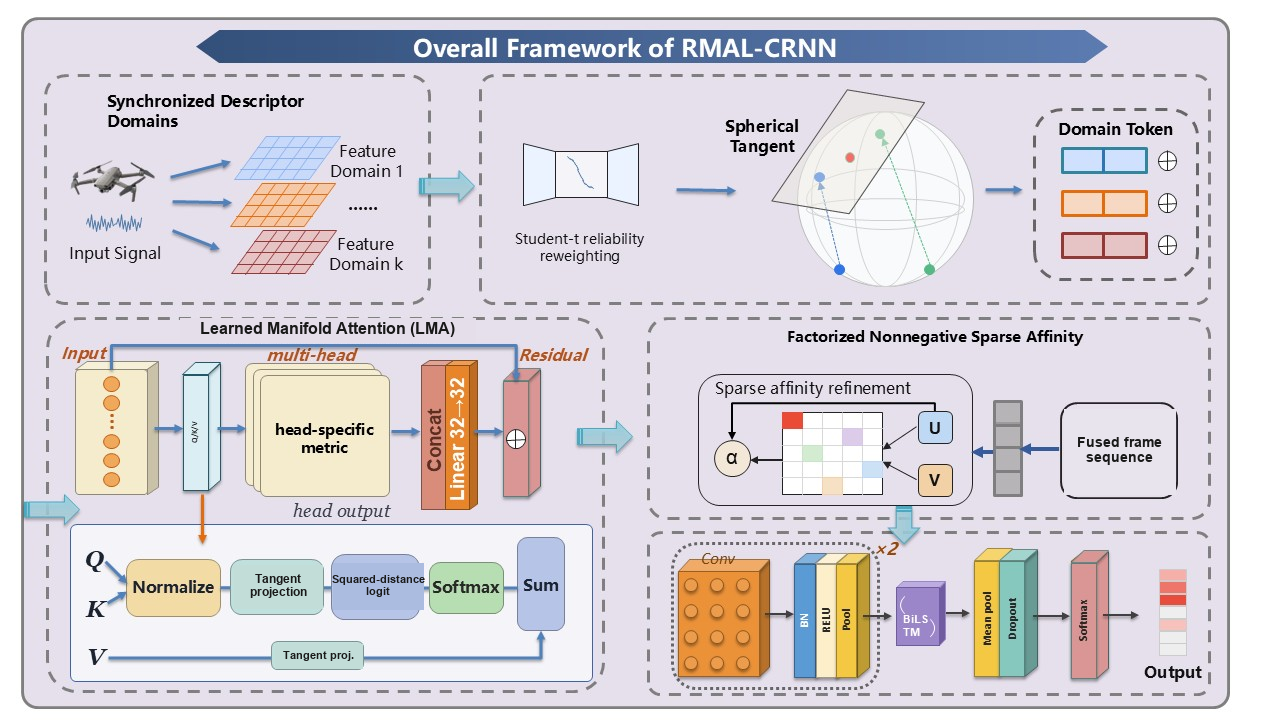
\includegraphics[width=\linewidth]{figures/fig1.png}
  \caption{Ordered RMAL-CRNN path. Coordinate reliability precedes domain-specific tangent projection and cross-domain relation learning. The fused frame sequence then parameterizes learned factors for temporal affinity refinement.}
  \label{fig:framework}
\end{figure}

\subsection{Geometric Student-t Tangent-Subspace Projection (GST)}
Heavy-tailed deviations motivate a Student-$t$-shaped reliability score \citep{lange1989student}. For domain $k$, learn a center $\boldsymbol\mu_k\in\R^d$, scale parameters $\boldsymbol\alpha_k\in\R^d$, and log-inverse degrees of freedom $\boldsymbol\eta_k\in\R^d$. Coordinatewise, $\boldsymbol\sigma_k=\max(\exp(\boldsymbol\alpha_k),\epsilon\mathbf1)$ and $\nu_{k,j}=1/\operatorname{clip}(e^{\eta_{k,j}},10^{-4},1)$. With stabilizer $\epsilon>0$, all-ones vector $\mathbf1$, elementwise division $\oslash$, and Hadamard product $\odot$, the standardized residual $\boldsymbol\rho_t^{(k)}$, reliability vector $\mathbf g_t^{(k)}$, and corrected block $\widehat{\mathbf x}_t^{(k)}$ are
\begin{align}
\boldsymbol\rho_t^{(k)}
&=(\mathbf x_t^{(k)}-\boldsymbol\mu_k)
\oslash\boldsymbol\sigma_k,\nonumber\\
\mathbf g_t^{(k)}
&=(\boldsymbol\nu_k+\mathbf1)\oslash
\left(\boldsymbol\nu_k+\boldsymbol\rho_t^{(k)}\odot\boldsymbol\rho_t^{(k)}\right),\nonumber\\
\widehat{\mathbf x}_t^{(k)}&=\mathbf g_t^{(k)}\odot\mathbf x_t^{(k)}.
\label{eq:gst-gate}
\end{align}
Here $\boldsymbol\nu_k=(\nu_{k,1},\ldots,\nu_{k,d})^\top$ and $\epsilon=10^{-6}$. Each entry satisfies $0<g_{t,j}^{(k)}\leq1+1/\nu_{k,j}$: coordinates near the learned center retain or mildly increase their weight, while large standardized residuals are attenuated.

For the equal-dimensional blocks used here, the corrected block is projected directly by $\Pi_{\mathbf p_k}$:
\begin{align}
\mathbf h_t^{(k)}&=\widehat{\mathbf x}_t^{(k)},
&\mathbf h_t^{(k)}&\in\R^d,
\label{eq:domain-alignment}\\
\mathbf p_k&=\frac{\overline{\mathbf p}_k}{\max(\|\overline{\mathbf p}_k\|_2,\epsilon)},
&\Pi_{\mathbf p_k}&=\mathbf I_d-\mathbf p_k\mathbf p_k^\top,
\label{eq:domain-basepoint}\\
\mathbf u_t^{(k)}&=\Pi_{\mathbf p_k}\mathbf h_t^{(k)}.
\label{eq:tangent-projection}
\end{align}
The projected component $\mathbf u_t^{(k)}$ lies in the tangent plane. The implementation then normalizes it and adds an unconstrained learned domain bias $\mathbf b_k$:
\begin{equation}
\mathbf z_t^{(k)}
=\sqrt d\,\frac{\mathbf u_t^{(k)}}{\max(\|\mathbf u_t^{(k)}\|_2,\epsilon)}
+\mathbf b_k.
\label{eq:token}
\end{equation}
Stacking gives $\mathbf Z_t=[\mathbf z_t^{(1)},\ldots,\mathbf z_t^{(K)}]^\top\in\R^{K\times d}$. Appendix~\ref{app:blockwise} proves blockwise directional agreement with the spherical logarithmic map on the unit-normalization branch $\|\overline{\mathbf p}_k\|_2\geq\epsilon$. The normalized component lies in its tangent space; adding $\mathbf b_k$ yields an affine tangent token.

\subsection{Learned Manifold Attention (LMA) with Tangent Metrics}
We add an unconstrained learned domain embedding $\mathbf e_k$ to retain source identity, $\widetilde{\mathbf z}_t^{(k)}=\mathbf z_t^{(k)}+\mathbf e_k$. For head $h\in\{1,\ldots,N_h\}$, let $d_h=d/N_h$, normalize a learned base point $\mathbf p_h$ with the same $\epsilon$ safeguard, and set $\Pi_{\mathbf p_h}=\mathbf I-\mathbf p_h\mathbf p_h^\top$. The matrices $\mathbf W_q^h$, $\mathbf W_k^h$, and $\mathbf W_v^h$ are learned query, key, and value maps. Queries and keys are normalized before projection; values are projected into the same head tangent plane. The tangent interpretation uses unit base points; the residual and LayerNorm operate in the ambient feature space:
\begin{equation}
\begin{aligned}
\overline{\mathbf q}_i^h&=\frac{\mathbf W_q^h\widetilde{\mathbf z}_t^{(i)}}
{\max(\|\mathbf W_q^h\widetilde{\mathbf z}_t^{(i)}\|_2,\epsilon)},
&\mathbf q_i^h&=\Pi_{\mathbf p_h}\overline{\mathbf q}_i^h,\\
\overline{\mathbf k}_j^h&=\frac{\mathbf W_k^h\widetilde{\mathbf z}_t^{(j)}}
{\max(\|\mathbf W_k^h\widetilde{\mathbf z}_t^{(j)}\|_2,\epsilon)},
&\mathbf k_j^h&=\Pi_{\mathbf p_h}\overline{\mathbf k}_j^h,\\
\mathbf v_j^h&=\Pi_{\mathbf p_h}\mathbf W_v^h\widetilde{\mathbf z}_t^{(j)}.
\end{aligned}
\label{eq:qkv}
\end{equation}
Instead of a dot product, the logit is the negative squared distance induced by the flat metric of the learned tangent plane:
\begin{align}
\ell_{ij}^h&=-\gamma_h\|\mathbf q_i^h-\mathbf k_j^h\|_2^2,
&\gamma_h&=\exp(\overline\gamma_h)>0,
\label{eq:attention-logit}\\
a_{ij}^h&=\frac{\exp(\ell_{ij}^h)}{\sum_{m=1}^{K}\exp(\ell_{im}^h)}.
\label{eq:attention-weight}
\end{align}
With output map $\mathbf W_o$ and LayerNorm operator $\LN$, the attended tokens $\mathbf y_{t,i}$ are
\begin{equation}
\mathbf y_{t,i}=\LN\!\left(\widetilde{\mathbf z}_t^{(i)}+
\mathbf W_o\operatorname{concat}_{h=1}^{N_h}
\sum_{j=1}^{K}a_{ij}^h\mathbf v_j^h\right).
\label{eq:attention-output}
\end{equation}

Normalization and orthogonal projection imply 
$\|\mathbf q_i^h-\mathbf k_j^h\|_2^2\leq4$. Hence the logits are bounded in $[-4\gamma_h,0]$, and Appendix~\ref{app:attention-proof} gives a finite-bandwidth upper bound on the largest attention weight and a corresponding entropy lower bound. The head base point removes one learned direction from each preprojected difference:
\begin{equation}
\|\Pi_{\mathbf p_h}(\overline{\mathbf q}-\overline{\mathbf k})\|_2^2
=\|\overline{\mathbf q}-\overline{\mathbf k}\|_2^2
-\big((\overline{\mathbf q}-\overline{\mathbf k})^\top\mathbf p_h\big)^2.
\label{eq:head-geometry}
\end{equation}
Different heads therefore learn complementary rank-$(d_h-1)$ metrics. The distinction from standard attention \citep{vaswani2017attention} is the learned tangent projector and its squared-distance kernel in that plane, not attention as a general operation.

\subsection{Factorized Nonnegative Sparse Affinity Refinement (FNSAR)}
After concatenating the $K$ attended tokens, a QR-initialized learned linear map yields one frame vector $\mathbf f_t\in\R^{d_f}$, and $\mathbf F=[\mathbf f_1,\ldots,\mathbf f_T]^\top$. Learned factor maps $\mathbf W_u,\mathbf W_v\in\R^{r_\ell\times d_f}$ construct a directed temporal relation with rank budget $r_\ell$:
\begin{equation}
\begin{alignedat}{2}
\mathbf U&=\mathbf F\mathbf W_u^\top &\quad&\in\R^{T\times r_\ell},\\
\mathbf V&=\mathbf F\mathbf W_v^\top &&\in\R^{T\times r_\ell},\\
\mathbf C_{\mathrm{raw}}&=r_\ell^{-1/2}\mathbf U\mathbf V^\top &&\in\R^{T\times T},\\
\mathbf C&=\ReLU\!\left(\mathbf C_{\mathrm{raw}}-\vartheta\mathbf1\mathbf1^\top\right),
&&\vartheta=\exp(\overline\vartheta)>0.
\end{alignedat}
\label{eq:fnsar-affinity}
\end{equation}
Here $\mathbf1\mathbf1^\top\in\R^{T\times T}$, $\ReLU$ acts entrywise, and the learned positive threshold is $\vartheta$. The raw affinity satisfies $\rank(\mathbf C_{\mathrm{raw}})\leq r_\ell$. Entrywise thresholding is the proximal map of a nonnegative $\ell_1$ penalty: at fixed $\mathbf C_{\mathrm{raw}}$, increasing $\vartheta$ removes support. The rank budget applies to the raw factorized relation; thresholding controls the support of $\mathbf C$. The refined output retains a direct residual path, with logistic sigmoid $\sigma$ setting the learned mixing coefficient $\zeta$:
\begin{equation}
\mathbf f_t^{\mathrm{out}}
=(1-\zeta)\mathbf f_t+
\zeta\,\LN\!\left(\sum_{s=1}^{T}C_{ts}\mathbf f_s\right),
\qquad \zeta=\sigma(\overline\zeta)\in(0,1).
\label{eq:fnsar-output}
\end{equation}
Appendix~\ref{app:affinity} proves the rank, proximal-support, and LayerNorm-residual bounds. This construction is related to differentiable self-expression \citep{elhamifar2013ssc,liu2013lrr,ji2017dsc}, but operates on the already fused temporal sequence and explicitly enforces nonnegative sparse support.

\subsection{Training and Cost}
The output sequence is classified by a CRNN. With label-smoothed cross-entropy $\mathcal L_{\mathrm{cls}}$, factor and sparsity weights $\lambda_{\mathrm{fac}}=\lambda_{\mathrm{sps}}=10^{-3}$, and elementwise squaring, training minimizes
\begin{equation}
\mathcal L=\mathcal L_{\mathrm{cls}}
+\frac{\lambda_{\mathrm{fac}}}{2}
\left[\operatorname{mean}(\mathbf U\odot\mathbf U)+\operatorname{mean}(\mathbf V\odot\mathbf V)\right]
+\lambda_{\mathrm{sps}}\operatorname{mean}(|\mathbf C|).
\label{eq:objective}
\end{equation}
Here $\operatorname{mean}$ averages every entry, including the minibatch dimension, and the cross-entropy uses smoothing $0.1$. The cross-domain attention costs $O(TK^2d)$ after linear projections. Temporal affinity formation and aggregation cost $O(T^2r_\ell)$ and $O(T^2d_f)$; the method remains quadratic in sequence length but avoids iterative singular-value decomposition. Appendix~\ref{app:implementation} records the complete configuration and hyperparameter study.
